\chapter*{章末习题答案}
\addcontentsline{toc}{chapter}{章末习题答案}
\markboth{章末习题答案}{章末习题答案}
\sourcepage{643}
\section{第 1 章\quad 起步：临床研究的结构与运作}
\begin{answerlist}
\item[1a.] 这是内部效度推断，因为涉及本研究中的妇女，很可能有效。但若母乳喂养率的差别由早期少量配方奶（ELF）以外的因素造成，例如对照干预对母乳喂养有不良影响；若自报情况不反映实际喂养；或关联由偶然性造成，推断也可能无效。显著的 $P$ 值不能排除这种可能。事实上，后续更大研究未重复得到这一阳性发现：Flaherman VJ, Narayan NR, Hartigan-O’Connor D, Cabana MD, McCulloch CE, Paul IM. The effect of early limited formula on breastfeeding, readmission, and intestinal microbiota: A randomized clinical trial. \textit{J Pediatr}. 2018;196:84-90 e1。
\item[1b.] 这是外部效度推断，因为推广到研究之外，可能有效。但除了内部效度的威胁同样也威胁外部效度，社区医院及国内其他地区产妇可能对干预反应不同；其他医师实施 ELF 的方式可能与原研究不同；或获益不能持续至 6 个月。
\item[1c.] 这一外部效度推断远超研究的人群和干预，很可能无效。它不仅推广到其他地区的母亲与新生儿，还纳入体重未下降 5\% 的新生儿；把早期少量补充扩展为无限制提供配方奶；并声称广泛而含糊的健康益处。后者虽可能合理，却没有在 ELF 研究中检验。
\item[2a.] 这是一项队列研究，研究温斯顿-塞勒姆高中生观看电视摔角节目，是否预测随后打架。
\item[2b.] 这是一项病例对照研究，研究曾至少母乳喂养一个孩子的中国妇女中，喂养持续时间是否与卵巢癌风险降低相关。
\item[2c.] 这是一项横断面研究，研究接受征兵体检的丹麦男性自报饱和脂肪摄入与精子浓度的关系。
\item[2d.] 这是一项随机试验，研究因其他原因接受心脏手术的心房颤动成人中，左心耳封堵相较不封堵，是否降低卒中或全身性栓塞发生率。
\end{answerlist}
这四句话均通过设计和研究问题的主要要素——关键变量与预定样本——简明概括整个研究。例如 2a 的设计是队列研究，预测因素是观看电视摔角节目，结局是打架，预定样本是温斯顿-塞勒姆高中生。

\section{第 2 章\quad 构思研究问题与制订研究计划}
\begin{answerlist}
\item[1.] 从研究问题走向计划，常需反复调整。最初可能写：“一项横断面研究，确定年轻成人中大麻使用是否与健康状况相关。”这一可能的联系似乎重要，但问题仍太模糊，无法判断可行性、新颖性和伦理性。\sourcepage{644}如何测量大麻使用与健康状况，目标人群是什么？横断面研究也难以确立因果：大麻使健康变差，还是反之？

更具体、也更符合 FINE 标准（可行、重要、新颖、符合伦理）的版本，可以是：“一项队列研究，确定大学三年级学生中，每天使用大麻者与不用者相比，随后一年因疾病到学生健康服务机构就诊的次数是否不同。”
\item[2.] 对乙酰氨基酚与哮喘的例子中，两者在全球同时增加的观察，以及该药耗竭还原型谷胱甘肽这一生物学合理性，使各项研究都有意义、值得关注；但随着研究增多，新颖性会减少。

\textbf{研究 1：}病例对照研究，比较伦敦南部全科诊所有哮喘症状成人（病例）自报使用对乙酰氨基酚的频率，与同一诊所随机选择、无该症状成人（对照）的频率。病例对照常适于开始探索关联（第 9 章）。本研究是一项探讨膳食抗氧化剂的、更大的人群基础哮喘病例对照研究的一部分，因而可行。哮喘与该药使用相关，每天使用者的比值比为 2.4（95\% CI：1.2—4.6）。作为不使参与者承担风险的观察性研究，它符合伦理。见 Shaheen SO, Sterne JA, Songhurst CE, Burney PG. Frequent paracetamol use and asthma in adults. \textit{Thorax}. 2000;55:266-270。

\textbf{研究 2：}多国横断面研究，由父母报告 6—7 岁儿童的过敏症状，包括哮喘、花粉症、湿疹，同时询问过去一年该药使用，以及出生第一年发热时通常是否使用。来自 31 国 73 中心的 205\,487 名儿童，若非纳入更广泛的国际儿童哮喘与过敏研究（ISAAC），本研究不可能完成。这说明探索新问题时，寻找已有数据或研究很重要（第 16 章）。当前使用与喘息有明显剂量－反应关系；对“孩子出生后前 12 个月，通常是否用扑热息痛〔对乙酰氨基酚〕退烧”答“是”者，喘息比值比为 1.46（95\% CI：1.36—1.56）。见 Beasley R, Clayton T, Crane J, et al. Association between paracetamol use in infancy and childhood, and risk of asthma, rhinoconjunctivitis, and eczema in children aged 6-7 years: analysis from Phase Three of the ISAAC programme. \textit{Lancet}. 2008;372:1039-1048。

\textbf{研究 3：}随机双盲试验，纳入登记时正在接受哮喘治疗的 6 月龄至 12 岁发热儿童，比较对乙酰氨基酚（12 mg/kg）与布洛芬（5 或 10 mg/kg）对四周内哮喘住院和门诊就诊的影响。随机试验费用与组织负担较高，通常最不易实施。潜在药物不良作用的资料越多，再随机验证也越不符合伦理。本研究回顾分析 1993 年已结束招募的波士顿大学发热研究中哮喘儿童亚组；该研究本为随机双盲试验。随机接受对乙酰氨基酚者，哮喘门诊风险较高，住院风险却没有增加。见 Lesko SM, Louik C, Vezina RM, Mitchell AA. Asthma morbidity after the short-term use of ibuprofen in children. \textit{Pediatrics}. 2002;109:E20。
\item[3.] 与同事分享你的答案！
\end{answerlist}

\sourcepage{645}
\section{第 3 章\quad 选择研究参与者：界定、抽样与招募}
\begin{answerlist}
\item[1a.] 如果吸烟的前因出现得更早，十一年级样本就未必适合研究问题，初中生可能是更有意义的目标人群。单所高中这一可接触人群，也未必代表目标人群，因为吸烟原因随文化情境而异；从全地区随机选若干高中可能更好。最重要的是，招募志愿者的设计，在吸烟行为上很可能不能代表可接触人群。
\item[1b.] 缺乏代表性可能来自随机误差，但除非样本很小，否则不太可能。例如，10 人样本中，偶然出现 $7:3$ 并不少见：从男女各半的大班抽 10 人，至少七名女生的概率约 17\%，至少七名男生也约 17\%。若样本为 100 人，至少 70 名女生的概率则小于 0.01\%。这说明取得样本后，可以估计抽样误差中随机部分的大小，也可通过扩大样本将它减到任何需要的程度。

也可能是系统误差：女生较多，可能因男女参与率不同。防止无应答偏倚的方法，包括各种提高招募率的措施；也可能是列出或抽取姓名时出错，需适当使用预试和质量控制（第 18 章）。
\item[2a.] 随机样本，属于概率抽样。可推广性的主要问题是无应答，问卷应短，并提供填写激励。本题所有抽样方法都可能有无应答偏倚。
\item[2b.] 分层随机样本，属于概率抽样；对女性超额抽取三倍，也许因为预期女性较少参加音乐会。
\item[2c.] 系统样本，属于非概率抽样。虽然方便，却会使情侣双方共同入选不足。至少理论上，售票员还可操控谁拿到尾号为 1 的票。
\item[2d.] 整群样本，属于概率抽样。可能方便，但同排座位的人可能比随机选的观众更相似，分析需考虑聚集性。若某些排音量更大，尤其可能有问题。
\item[2e.] 连续样本，属于非概率抽样。通常是好选择，但早到者与晚到者可能不同，故在不同时段各取连续样本更好。
\item[2f.] 便利样本，属于非概率抽样。会漏掉邮购票者，成组参加者也可能被过多或过少代表。
\item[2g.] 便利样本，属于非概率抽样。除受研究者随意选择影响外，还可能因观众听不到邀请而无应答。
\sourcepage{646}
\item[3a.] 目标人群是研究时期美国全体 5 岁以下儿童，因为作者用全国调查估计美国人偏肺病毒（HMPV）的疾病负担。当然也希望推广到未来，许多读者会不假思索这样做；但特别对年际频率变化的传染病，推广到研究年份之外，是额外且可能脆弱的推断。
\item[3b.] 可接触人群是居住于三个研究地点——辛辛那提、纳什维尔、纽约州罗切斯特——周边县，并在研究机构就诊的 5 岁以下儿童。选择这些城市，大概因为靠近研究者；它们在 HMPV 感染频率上能在多大程度上代表美国其他地区，并不清楚。
\item[3c.] 是便利抽样。未说明选择一周哪些日子；若轻症儿童家长周末等到周一才就医，而 HMPV 症状又比其他病毒重或轻，就可能有偏倚。在招募日，研究者也许尝试连续抽样（同样未说明），可帮助控制选择偏倚。限制某些月份的原因未交代，大概认为病例几乎均出现在这些月份。
\item[3d.] 观察按地理区域聚集，统计需考虑。城市间估计越不同，区间越宽；直觉上也合理：各市发病率差别越大，就越会怀疑若纳入其他城市，估计又会怎样，这种不确定性应反映为更宽的区间。

更隐蔽的聚集单位是年份。如果 HMPV 发病率年际变化很大，又想推广到未来而不只是估计研究年份，就需考虑按年份聚集；年际变异也会使区间更宽。
\end{answerlist}

\section{第 4 章\quad 规划测量：精密度、准确度与效度}
\begin{answerlist}
\item[1a—i.] 依次为：二分类；连续；二分类；名义；离散数值；有序；连续；名义；二分类。
\end{answerlist}
结局包含有序信息，通常可提高效能。例如，将教育测为最高年级或总受教育年数，比二分为有无大学学历更有力。把体重指数作连续结局，也比有无肥胖，或体重过低／正常／超重／肥胖这一有序分类包含更多信息、效能更高。
\sourcepage{647}
\begin{answerlist}
\item[2a.] 这是仪器变异造成的系统误差。需更换校准用的 10 kg 砝码，否则以后会系统性低估婴儿体重。但若所有婴儿均用同一台秤，对“6 月龄果汁摄入多能预测 1 岁体重”仍可给出无偏答案。
\item[2b.] 是精密度问题，最可能来自仪器变异。过大变异也可能是观察者错误，尤其非数字秤，但更可能需换秤或电池。
\item[2c.] 两类误差都可能有。婴儿扭动程度及影响不同，导致不精密；观察者扶抱改变示数，造成系统误差，方向取决于抱法。可由母亲安抚；若成人秤足够准确，也可分别称母亲抱婴儿与不抱时的体重，取差值。
\item[2d.] 主要是精密度问题：若秤准确，示数会围绕真实体重波动。变异来自参与者，解决方法同 2c。
\item[2e.] 主要是精密度问题，体重随检查前进食或尿湿纸尿裤而变。可指导母亲检查前三小时不喂食，并让婴儿裸身称重。若观察者处理湿尿裤方式不同——脱下、更换或不处理——也会有观察者变异。
\item[3a.] 预测效度：倦怠评分预测了预期与倦怠有关的结局。
\item[3b.] 表面效度：熟悉倦怠者认为这种评价方式合理。
\item[3c.] 构念效度：指标对预期会影响倦怠的情境有所反应。
\item[3d.] 效标关联效度：这两项与公认标准测量高度一致。
\end{answerlist}

\section{第 5 章\quad 样本量估计的准备：假设与基本原理}
\begin{answerlist}
\item[1.] \textbf{样本量：}研究纳入的参与者人数。估算应指向完成研究且有数据可分析的人数。分析性研究中，可根据指定 $\alpha$ 与 $\beta$ 下检出给定效应量所需人数来估计。

\textbf{零假设：}说明比较组间无差异的研究假设表述。

\textbf{备择假设：}说明比较组间有差异的研究假设表述。

\textbf{检验效能：}若人群真实差异等于规定效应量，在给定样本量与显著性水平下，检出统计学显著组间差异的概率。

\textbf{统计学显著性水平：}零假设为真时，事先设定的错误拒绝概率。
\sourcepage{648}
\textbf{效应量：}研究者希望以合理机会检出的组间最小差异。

\textbf{变异性：}测量的分散程度，通常用标准差表示。
\item[2a.] 两者都不是。结果有统计学显著性，没有理由认为是 I 类错误。
\item[2b.] 样本小，研究期发生肺癌者很少。尤其已有大量吸烟致肺癌的其他研究，这一阴性结果几乎肯定是 II 类错误。
\item[2c.] 事先没有流行病学或病理生理学理由认为饮酒降低糖尿病风险，结果可能是 I 类错误。研究者可给更多信息：$P<0.05$ 既可能为 0.04，也可能为 0.001；后者会降低、但不能排除 I 类错误的可能。
\end{answerlist}

\section{第 6 章\quad 估计样本量：应用与实例}
\begin{answerlist}
\item[1.] $H_0$：胃癌病例与对照的体重指数无差异。\\
$H_A$（双侧）：胃癌病例与对照的体重指数有差异。

体重指数是连续变量，病例／对照状态是二分类变量，因此可用 $t$ 检验。效应量 $E=1$ kg/m$^2$，标准差 $S=2.5$ kg/m$^2$，$E/S=0.4$。查附录 6A：
\begin{itemize}
\item $\alpha$（双侧）$=0.05$，$\beta=0.20$，每组需 100 人。
\item $\alpha$（双侧）$=0.05$，$\beta=0.10$（效能 0.9），每组需 133 人。
\item $\alpha$（双侧）$=0.01$，$\beta=0.20$，每组需 148 人。
\end{itemize}
\textbf{加分题：}第 6 章建议的方法如下。
\begin{enumerate}
\item 使用连续变量：体重指数已经连续，病例／对照状态不能改为连续。
\item 使用更精密的变量：身高体重本已较精密，体重指数标准差主要是不能减小的个体间变异。规范测量仍有用，但不是最佳选择。
\item 配对测量：不适用，研究体重指数“变化”会变成另一个问题。
\item 使用更常见结局：不适用于病例对照研究。
\item 组间人数不等：容易找到无胃癌者，可以增加对照。例如，每例配四名对照，对照共 240 人，可用第 6 章近似式
\[
n'=\left(\frac{c+1}{2c}\right)n,
\]
其中 $n'$ 为新病例数，$c$ 为对照／病例比（本例为 4），$n$ 为按 $1:1$ 时的原病例数。\sourcepage{649}因此
\[
n'=\frac{4+1}{8}\times100=\frac58\times100=63,
\]
接近可用病例数。60 病例、240 对照的效能，与各 100 人相近但略低。
\end{enumerate}
\item[2.] $H_0$：DHEA 治疗与安慰剂组平均力量无差异。\\
$H_A$：两组平均力量有差异。\\
$\alpha$（双侧）$=0.05$，$\beta=0.10$。\\
效应量 $=10\%\times20$ kg $=2$ g\footnote{译注：底本此处写作 2 g；按同一行的 $10\%\times20$ kg 计算应为 2 kg，且后面的 $E/S=0.25$ 也按 2 kg 得到。此处保留原单位以标明底本差异。}，标准差为 8 kg，$E/S=0.25$。

用 $t$ 检验比较，查附录 6A 左列 0.25，再移到左起第五列（双侧 $\alpha=0.05$、$\beta=0.10$），每组约 338 人。若 $\beta=0.20$，每组 253 人。
\item[3.] $H_0$：DHEA 与安慰剂组力量平均变化无差异。\\
$H_A$：两组力量平均变化有差异。\\
$\alpha$（双侧）$=0.05$，$\beta=0.10$，效应量 $=10\%\times20$ kg $=2$ kg，标准差 2 kg，$E/S=1.0$。

查附录 6A 左列 1.00，再移到左起第五列，每组约需 23 人。
\item[4.] $H_0$：有、无阅读障碍学生的左利手频率无差异。\\
$H_A$：两组左利手频率有差异。\\
$\alpha$（双侧）$=0.05$，$\beta=0.20$，效应量为比值比 2.0。

无阅读障碍者左利手比例 $P_0$ 约为 0.1，要检出使比值比为 2 的阅读障碍者比例 $P_1$。使用卡方检验，查附录 6B；但表输入的是两个比例，而非比值比，目前只知 $P_0=0.1$。用第 6 章公式：
\[
P_1=\frac{\mathrm{OR}\times P_0}{(1-P_0)+(\mathrm{OR}\times P_0)}.
\]
\sourcepage{650}
本例为
\[
P_1=\frac{2\times0.1}{(1-0.1)+(2\times0.1)}
=\frac{0.2}{0.9+0.2}=0.18.
\]
两比例用卡方检验比较；$P_1-P_0=0.18-0.10=0.08$。附录 6B 表 6B.2 给出每组需 318 人。
\item[5.] 虽然 IQ 测验标准差通常为 15，医学生分布较窄也合理。标准差约为“通常”范围的四分之一，即 $(150-110)/4=10$ 分。置信区间总宽 6 分，上下各 3；标准化宽度 $W/S=6/10=0.6$，置信水平 99\%。查表 6D 的 $W/S=0.60$、99\% 列，约需 74 名医学生，才能得到均值区间 $\pm3$ 分。
\end{answerlist}

\section{第 7 章\quad 处理伦理问题}
\begin{answerlist}
\item[1a.] 从伦理看，若原研究同意涵盖未来研究（含 DNA 测序），或对未明确的未来研究给予广泛同意，拟议研究当然可以依据原同意开展。但原同意也可能含糊，例如“可与从事相关研究者共享”，或未提未来研究；此时 IRB 可判断二次项目是否属于原同意范围。
\item[1b.] 对原同意过于严格的解释，会阻止有价值的二次研究；它们可能增进疾病知识、不伤害参与者，而重新收集标本又极困难。拟议研究无额外医学风险。但基因组测序可能被区别对待，不同于在存储标本上验证糖尿病或冠心病新生物标志物等实验。保密一旦破坏，参与者可能被污名化、隐私丧失或受歧视，因此需适当保密措施。

即使原同意未涵盖，也有办法：IRB 可按相应标准豁免知情同意；更常见的是，持有者移除病历号等明显标识，以数字代码连接标本与数据，代码钥匙销毁，或不向二次研究者提供。但若原同意明确说不会与其他研究者共享标本，移除标识后这样研究，仍有伦理问题。
\item[1c.] 采集新标本时，宜征求额外收血储存用于未来研究的许可，比重建队列高效。推荐分层同意：分别同意（1）特定研究，如原队列；（2）同一大主题其他项目，如冠心病或卒中风险；（3）任何获 IRB 及科学评审组批准的未来研究。针对 1b，还可专门征求 DNA 测序同意。\sourcepage{651}参与者可同意一项、两项或全部。当然，未来研究无法充分描述，因此从不知道其性质、风险与获益的意义上说，并非真正充分知情；参与者是信任 IRB 和科学评审组只会允许科学与伦理上适当的研究。NIH 正拟定未来标本使用同意的考虑事项及示例语言，见 \url{https://grants.nih.gov/grants/guide/notice-files/NOT-OD-21-131.html}。
\item[2a.] 对照组不给已知能改善重要临床结局的药物，会使参与者承受不正当伤害，因此不符合伦理。即使本人同意，IRB 也不应批准，因为不满足风险－获益可接受及尽量减小风险的监管要求。
\item[2b.] 可先让全部患者接受现行标准化疗，再随机给予新治疗或安慰剂。或寻找尚无治疗被证明能延长生存的亚组；生存是肿瘤最重要的临床终点。例如，经多种标准化疗仍进展、再无已证有效选择者，可参加实验干预的安慰剂对照试验。这假定其他治疗失败后有效的药，也会在未治疗者有效；当然，难治病例无效的药，也可能作为一线治疗有效。与安慰剂对照相比，这些设计效能较低。
\item[3a.] 资源丰富国家的资助者和研究者，在资源不足国家研究时，可能利用弱势参与者及国家。伦理上最好的安排是：由在当地实际提供医疗、受信任的人道组织，例如无国界医生，与无利益冲突的东道国研究者合作，开展可行性研究及后续试验；获所在国政府及非政府服务组织批准。为保证居民长期获益，应在可行性试验前协商协议，使该国能切实获得疫苗，例如以可负担价格提供有意义的数量。\footnote{译注：底本答案 3a 讨论资源不足国家的研究安排，与第 7 章习题 3a 的信息披露问题不对应。底本答案 3b、3c 分别讨论信息披露与理解，降低 HIV 感染风险的讨论则接在 3c 后。本译本保留底本顺序。}
\item[3b.] 知情同意应讨论：（1）研究性质；（2）访视次数与时长；（3）参与的潜在获益与风险，本例主要是泄密后的污名及歧视；（4）不参与的替代选择，包括试验外已有或可能提供的 HIV 预防措施；（5）自愿参与及随时退出权；（6）符合州公共卫生报告要求的保密保护。
\item[3c.] 信息应以参与者能理解的方式呈现。健康素养较低者无法理解详细书面同意，可咨询社区与倡议团体，考虑视频、漫画等；对翻译并回译的材料充分预试，找出常见误解，再据此改进同意过程。
\sourcepage{652}
即使是观察性研究，也有伦理义务告知如何降低 HIV 风险；科学上和伦理上都有理由。研究者须预防对参与者的伤害，不能不给可行、已知能预防潜在致命研究终点的公共卫生措施，包括咨询、安全套、转介药物滥用治疗及针具交换。后续疫苗试验也必须提供，即使会降低效能。
\end{answerlist}

\section{第 8 章\quad 横断面研究与队列研究的设计}
\begin{answerlist}
\item[1a.] 先定纳入排除标准并招募样本，例如至少 70 岁且无髋骨折史者；测血清维生素 B$_{12}$ 和其他髋骨折预测因素，也可储存血清待用。伦理上，对明确缺乏 B$_{12}$ 者应治疗，并可能排除。随后随访，如五年，记录髋骨折，分析 B$_{12}$ 与新发骨折的关联。
\item[1b.] 优点是时间顺序明确，骨折前取得血清，有助于判断因果。骨折后可能因入住护理机构、摄入减少而 B$_{12}$ 降低；维生素 D 与日晒有关，问题可能更大。骨折后尽快取血可减轻这一顾虑。

缺点是需要成千上万人多年随访，昂贵且结果晚；期间饮食与补充剂变化，可能使起点水平不代表骨折时水平，需重复测量，增加复杂性与费用。
\item[1c.] 若有储存血清及较完整骨折随访的队列，可回顾研究，较省时省钱。主要缺点是长期储存可能改变 B$_{12}$ 测量，且可能缺少体力活动、吸烟等混杂因素。
\item[2a.] PRIDE 虽为随机试验，但起点检查的报告是观察性横断面研究。横断面研究常是队列或随机试验的第一步。
\item[2b.] 抑郁可能增加尿失禁，尿失禁也可能促成抑郁。还可能是偏倚，例如抑郁妇女并无更多发作，却更容易报告；\sourcepage{653}或肥胖等第三因素同时导致两者，形成混杂（第 10 章）。

纵向队列可澄清时间顺序：随访起点很少或无失禁的抑郁及非抑郁妇女，看抑郁者是否更易发生或加重；也可随访无抑郁史、不同失禁程度者，看失禁越多是否越易抑郁。暴露不止两级，可评价剂量－反应。最有说服力的是研究自然发生、或理想情况下由干预引起的改变，观察一者是否先于另一者：治好失禁后抑郁改善吗？抑郁消退后，报告的控尿能力改善吗？
\end{answerlist}

\section{第 9 章\quad 病例对照研究的设计}
\begin{answerlist}
\item[1.] 利用 8.1c 的队列，主要提高效率的方法是少测 B$_{12}$。不必在起点为全队列检测并治疗、排除低值者，而可先收血储存，再作巢式病例对照：测全部骨折病例及未骨折者随机样本。每例配四至五个对照，接近最高效率（原文指第 5 章“组间人数不等”的公式），比全体检测少得多。
\item[2a.] 最好在预定队列中纳入全部病例，作巢式病例对照。规定年龄，如 30—75 岁，以及最低诊断条件，如病理。若队列不够大，可由肿瘤登记找新近病例，限制为可电话联系且同意者。新近病例可减少只研究幸存者的偏倚；理想时还访谈死者亲属。
\item[2b.] 对照可从同一队列或登记所覆盖各县的 30—75 岁妇女中随机抽取。某些欧洲国家已有人口名册，较易随机；美国可能需要随机拨号，因此病例也应限于有电话者。
\item[2c.] 卵巢癌治疗强度大且可致死，部分病例不愿加入或访谈前已死。若家族史与更侵袭的癌相关，有家族史者较少活到入选，风险估计便偏低；若家族性癌预后较好，则相反。

健康妇女若家人患癌，可能更感兴趣、更愿作对照，使对照家族史比例偏高，\sourcepage{654}家族史的风险估计偏低。伦理允许时，不向潜在对照说明确切问题或具体癌种，可减轻这一问题。
\item[2d.] 询问有多少女性亲属及多少患卵巢癌来测家族史，可能有回忆偏倚。病例担心遗传易感，可能比无此顾虑的健康者更记得或主动了解亲属患病，关联估计偏高。

还可能混淆宫颈、子宫、卵巢癌及需手术的良性妇科肿瘤，造成暴露错分。无真实家族史者报告有危险因素；若病例与对照同等错分，比值比趋向 1。若病例更易误认亲属癌种或手术原因，则比值比偏高。查证被报告患癌亲属的病历，可减少错分。

还应考虑有阳性家族史的机会：姨姑和年长姐妹多者，比小家庭、仅有兄弟或妹妹者，机会更多。第 10 章的匹配与分层可处理。
\item[2e.] 最简单是二分家族史，例如有无一级亲属患病，以比值比衡量关联。卵巢癌罕见，因此近似相对风险，可用简单卡方显著性检验。若量化为一、二级女性亲属患病比例，也可分为家族史强度有序类别，计算各级比值比，寻找剂量－反应。全基因组关联研究（GWAS）还可识别病例中更常见的基因，但需大样本。
\item[2f.] 虽有抽样、回忆及错分问题，病例对照仍合理。另一选择是大型队列，但疾病太罕见，仅为这一问题开展队列大概不可行。若能找到已系统收集家族史的回顾性队列，则最理想。
\item[3a.] 病例可为撞车的年轻驾驶者，如 16—20 岁；对照为他们指出、未撞车的朋友或熟人。应排除一起玩电子游戏者，避免过度匹配。该年龄移动电话普遍，随机拨号寻找对照可能效果较差；也可用汽车保险公司记录寻找两组。年轻男性既更多玩游戏、也更多撞车，可考虑按性别匹配。用问卷或访谈测量游戏暴露，应问驾驶及非驾驶游戏，\sourcepage{655}若仅驾驶／竞速游戏而非射击或其他游戏有关，特异性会加强因果推断。
\item[3b.] 对驾驶前玩游戏这类假定有短期影响的间歇暴露，病例交叉研究很适合。病例同上，没有对照人，只有对照时段：询问撞车行程之前及未撞车的对照时段，是否玩竞速游戏。配对比较，看撞车前比其他时段是否更常玩。
\end{answerlist}

\section{第 10 章\quad 用观察性研究估计因果效应}
\begin{answerlist}
\item[1a.] 水果蔬菜摄入与冠心病（CHD）的观察关联，可能不代表因果效应，有四种原因。
\begin{itemize}
\item \textbf{偶然性。}患者摄入较少可能是随机误差。第 5 章指出，$P$ 值量化所见差异相对偶然预期有多大；95\% CI 显示与结果相容的取值范围。其他条件相同时，$P$ 值越小，置信区间中更靠近无效值的端点与无效值相距越远，偶然性就越不可能解释全部关联。
\item \textbf{偏倚。}样本、预测或结局可能有系统误差，即研究问题与实际实施系统性不同。例如，对照虽来自同一医保计划，却选自年度健康体检者；他们可能比全体风险人群更关注健康、多吃蔬果。心肌梗死者可能更易回忆不良饮食，造成回忆偏倚；不设盲访谈者也可能不同提问或记录。若多吃蔬果者的医生更积极或更不积极追查冠心病，结局测量也可能偏。
\item \textbf{果因倒置。}心肌梗死可能改变口味，减少蔬果。但更可能是受惊吓后多吃，反使保护作用看起来偏小。可研究时间顺序，例如问过去而非当前饮食，更好是把病例对照嵌入有事先饮食记录的队列。
\item \textbf{混杂。}多吃与少吃者有其他差异，真正导致冠心病率不同。例如多吃者也更多运动（见 1b）。
\end{itemize}
\item[1b.] 控制运动混杂的可能方法如下。
\end{answerlist}
\sourcepage{656}
\begingroup\small
\begin{longtable}{L{22mm}L{35mm}L{41mm}L{45mm}}
\toprule\textbf{方法}&\textbf{可能计划}&\textbf{优点}&\textbf{缺点}\\\midrule\endfirsthead
\toprule\textbf{方法}&\textbf{可能计划}&\textbf{优点}&\textbf{缺点}\\\midrule\endhead
\multicolumn{4}{l}{\textbf{设计阶段}}\\
规定条件&仅纳入自报无规律运动者。&简单。&限制合格人群，招募更难；可能不能推广到运动者。\\
匹配&每例匹配运动水平相近的对照。&消除运动对冠心病的预测作用，通常略提高观察饮食作用的精度与效能。&需额外寻找匹配者；无相近对照时浪费病例；失去研究运动作用的机会。\\
机会性研究&寻找影响蔬果摄入、但与冠心病无其他关联的外部因素，即工具变量。&若找到合适工具，可控制已测及未测混杂。&常难找到强且可信的工具。\\
\multicolumn{4}{l}{\textbf{分析阶段}}\\
分层&按运动分三、四层分析。&简单、易懂且可撤销重做。&只能合理处理少数层与混杂变量；连续运动改分类会丢信息，类别太宽还可能控制不完全。\\
统计调整（建模）&用 logistic 回归或 Cox 模型等，同时控制运动与其他混杂。&可保留运动连续变量全部信息，并同时控制年龄、种族／族裔、糖尿病、高血压、吸烟；调整可撤销。&模型可能不适合数据，导致残余混杂或误导。例如饮食或活动效应可能在吸烟者与不吸烟者不同；重要混杂须已测量。\sourcepage{657}尤其有交互作用或非二分类变量时，模型结果有时难理解、描述。\\\bottomrule
\end{longtable}\endgroup
除了上述观察性方法，还可设计随机试验；但可能须估计促进蔬果摄入干预的因果效应，而非摄入本身。

也值得寻找其他支持因果的依据：剂量－反应，如蔬果摄入越多，冠心病的比值越低；生物机制，如蔬果中的抗氧化剂保护动脉免于粥样硬化；以及跨人群、跨设计的一致性，如生态研究显示多吃蔬果的人群冠心病远少。
\begin{answerlist}
\item[2.] 这是对碰撞点、即共同结果条件化的例子。只纳入发热婴儿，而尿路与耳部感染均可引起发热。未环切男婴更易尿路感染，所以他们发热更可能由尿路而非耳部感染引起；即在无耳感染者中过多代表，也因在有尿路感染者中过多代表。
\item[3.] 可用队列研究：询问孕期对乙酰氨基酚使用，随访后代哮喘，寻找母亲基因型是否修饰暴露效应的依据，即在预测遗传易感性最高者中，暴露－结局关联更强的交互作用。已有这样的报告：Shaheen SO, Newson RB, Ring SM, Rose-Zerilli MJ, Holloway JW, Henderson AJ. Prenatal and infant acetaminophen exposure, antioxidant gene polymorphisms, and childhood asthma. \textit{J Allergy Clin Immunol}. 2010;126(6):1141-1148 e7。
\end{answerlist}

\section{第 11 章\quad 随机盲法试验的设计}
\begin{answerlist}
\item[1a.] 以生物标志物变化这一连续变量作主要结局，主要优点是样本量较小、时间较短，就能确定治疗是否降低标志物水平。主要缺点是不确定治疗导致的标志物变化，是否意味着真正减少远更重要的临床结局——痴呆发病。
\item[1b.] 临床确诊痴呆更有意义，可改善预防实践；但痴呆通常发展缓慢、发生人数少，因此试验可能规模大、耗时长且昂贵。
\item[2a.] 为尽量保留和随访参与者，起点应收集本人、密友、家人或医疗服务提供者的联系方式。
\item[2b.] 为便于他人评价样本的可推广性，收集年龄、种族／族裔、生理或社会性别等人口学资料、一般健康状况及起点认知损害程度。
\sourcepage{658}
\item[2c.] 为评价治疗效力，起点应实施全部效力结局测量，例如认知功能测验，或认知损害影响日常生活的其他指标。
\item[2d.] 为未来亚组分析，收集高血压、痴呆家族史、ApoE4 等位基因等危险因素或潜在效应修饰因素。它们可能识别结局率最高者，以便分组研究。
\item[2e.] 为未来尚未预见的问题，尽可能收集痴呆危险因素等资料，并储存血清或血浆，供以后测定影响疗效的因素，例如药物代谢酶基因型。也可请同事提出简便附属测量，例如起点额外问卷，以在试验样本中探索其他问题。
\item[3a.] 需纳入足够多的 ApoE4 携带者，使未来比较携带与不携带者石杉碱效应时有足够效能。故应在起点筛查，并富集携带者，达到总样本所需最低比例。可用分层区组随机化，使治疗与安慰剂组携带者人数相近。
\item[3b.] 若疗效确实随基因型明显不同，结果会有临床价值；但试验更复杂。入组前分型延迟随机化，并引出如何告知和咨询等问题。与不论基因型、只按资格招募相比，富集更难、更贵。随机方案复杂，也使各层药物与安慰剂准备、包装更难。因此，尚不知药物能否减缓痴呆进展的初次试验，可能决定暂不探索基因型差异。
\item[4a.] 这种方法省力省钱，却不大可能准确发现药物相关胃肠症状。长期试验结束时，患者可能记不清早期症状，也未必能最好判断是否由研究药物造成。
\item[4b.] 即使开始时鼓励报告，患者也可能忘记提及，所以会漏报。与方法 1 相似，若不认为症状由药物造成，也可能不报告。
\item[4c.] 这种方法较可能一致地获得腹泻、恶心及呕吐资料。部分症状虽无关，但可比较药物与安慰剂组的频率与严重程度，评价药物组是否更多、更重。
\item[4d.] 不仅可发现胃肠症状，也可能发现试验中许多其他症状或健康不良问题，\sourcepage{659}有助于发现意料外的不良作用。开放式回答可后续分类分析。不过，若要量化胃肠症状负担，应除一般开放式健康问题外，专门询问腹泻、恶心和呕吐。
\item[5.] 作为中期监察者，可要求症状严重程度与持续时间，判断潜在损害是否超过认知获益；也可查看发生症状者的特征，判断是否仅限某个以后可排除的亚组。可建议在后续筛查加入既往胃肠症状，如肠易激综合征，以免纳入更易发生严重反应者。
\item[6.] 意向治疗分析的主要缺点，是纳入未依从随机分配治疗者，使整个随机组的观察效应偏小。但用按实际治疗分析取代意向治疗分析，潜在缺点可能更大：未依从干预者通常在重要而未测量的方面不同于依从者，因此按实际治疗分析不再具有真正的随机比较，可能错误认定石杉碱有效。
\item[7.] 根据亚组分析声称年轻者更有效，可能只是偶然。总体不显著时，检验亚组越多，越可能找到“显著”结果，而这里未说明检验了多少组。声称 60 岁以下有效，暗示老年者无效甚至相反；也应报告并检验年龄是否修饰药物对认知损害的作用。如果分析是事后而非基于生物学理由预设，检验亚组很多，或治疗与年龄交互作用不显著，就应避免认定年轻亚组有效。
\end{answerlist}

\section{第 12 章\quad 其他干预性研究设计}
\begin{answerlist}
\item[1a.] HairStat 与安慰剂比较最简单、样本最小、费用最低，可明确判断是否优于安慰剂。但若非那雄胺已普遍用于男性型脱发，参与者可能在试验中使用它。即使双盲，HairStat 若有效，安慰剂组可能更易另用非那雄胺，使试验难以检出获益。可要求两组避免使用，但知道不能用已有有效药物，可能使一些人不愿参加。
\sourcepage{660}
\item[1b.] 若非那雄胺常用，比较两药可回答疗效是否不同这一重要问题。应先判断是否认为 HairStat 更有效；若是，可作比较效力试验，显示潜在优效。若认为同样有效但便宜得多，应考虑非劣效试验：纳入条件、剂量、时长和结局，应尽量类似确立非那雄胺效力的试验，并尽量减少不依从及失访。主要缺点是样本通常远大于安慰剂对照。
\item[1c.] 仅纳入曾用非那雄胺失败者，可避免上述问题：不想再用它，也无临床理由在这群人比较。但可能难招足够人数。不能耐受一种药者，也可能更不耐受另一种，即使机制不同。因此本试验的耐受问题频率或严重程度，可能高于既往非那雄胺报告，虽然在较少选择的人群中，两药不良事件可能相近。
\item[1d.] 含安慰剂的析因设计，可分别比较各药与安慰剂，并在效能足够时，检验联用是否优于单药；缺点是规模、成本和复杂性增加。
\item[1e.] 交叉试验使每人有机会使用各药，可能吸引参与。每人作自己的对照，也可比平行组小。但若停药后效应持续较久，换药后前几个月继续长发，就可能错归于下一种药。
\item[2a.] 个体随机似乎最简单，但工作场所干预难以甚至不可能只给同办公室部分人。例如公共区域海报人人可见，不论分组。因此，对这种办公室层面干预，个体随机大概不可行。
\item[2b.] 优点是所有员工和办公室均可获得干预，分析也简单：先收体重，全部同时实施，六个月后评价变化。但无对照，就难判断变化或不变是否归因于干预。\sourcepage{661}例如体重持平甚至稍增，可能被误判无效，其实无干预本会增得更多。中断时间序列可部分补救：考虑既有体重趋势，外推无干预轨迹。
\item[2c.] 逐步推广到所有办公室，较符合帮助全部超重肥胖员工减重的目标。但假定不论哪月开始，效果相同；实际可能有季节趋势，如冬季比春秋更易增重，使发现无效。
\item[2d.] 可严格比较随机选中实施与不实施的办公室。缺点是分析单位为办公室而非个人，需随机很多办公室才能有足够效能；各办公室大小不同、分析权重不同，也使分析复杂。
\end{answerlist}

\section{第 13 章\quad 医学检验研究的设计}
\begin{answerlist}
\item[1a.] 一般最好在尚不知谁有病时，从有风险者中抽样。本例可纳入因符合 PID 的腹痛到门诊或急诊者。最差是比较住院 PID 与健康对照：疾病谱，尤其非疾病谱，都不能代表实际临床人群。住院者病情可能更重，健康者 ESR 升高又远少于其他原因腹痛者。
\item[1b.] 若最终诊断者用 ESR 辅助判定，灵敏度和特异度都可能偏高；依赖越多，纳入偏倚越大。
\item[1c.] 最佳答案是不选单一异常界值，而用 ROC 曲线显示取舍，并报告各区间如 $<20$、20—49、$\geq50$ mm/小时的似然比。由题目可得：
\begin{center}\small
\begin{tabular}{lrrr}\toprule
ESR&有 PID&无 PID&似然比\\\midrule
$<20$&10\%&50\%&0.20\\
20—49&15\%&35\%&0.43\\
$\geq50$&75\%&15\%&5.00\\
合计&100\%&100\%&\\\bottomrule
\end{tabular}\end{center}
\sourcepage{662}
还可用 ROC 曲线与白细胞计数等检验比较。下列假想曲线提示，ESR 预测 PID 优于 WBC：
\begin{center}
\begin{tikzpicture}[x=.27mm,y=.27mm]
\node[anchor=south west,inner sep=0] at (0,0)
 {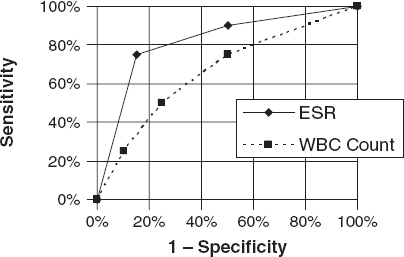
\includegraphics[width=109.08mm]{assets/answers_ch13_roc_original.png}};
\fill[white] (-3,40) rectangle (20,222);
\node[rotate=90,font=\small] at (9,145) {灵敏度};
\fill[white] (159,-2) rectangle (294,21);
\node[font=\small] at (223,10) {$1-$特异度};
\fill[white] (294,101) rectangle (401,154);
\node[anchor=west,font=\small] at (296,143) {ESR};
\node[anchor=west,font=\small] at (296,112) {WBC 计数};
\end{tikzpicture}
\end{center}
\item[2a.] 这是从分子排人、却不从分母排人的常见错误。虽仅 10 名儿童有“意外”异常，分母却应仅为神经检查及精神状态正常、异常才算意外者，可能远少于 200。若只有 100 人符合，检出率为 $10/100=10\%$，高一倍。
\item[2b.] 许多“异常”可能无临床意义。除非改变处理，而且能估计处理对结局的作用，否则难知多高检出率才值得。更好结局是“需要干预的颅内损伤”，但需对哪些损伤需干预达成共识，并估计干预改善结局的效果。
\item[2c.] 第一，可评价正常结果的好处，例如从住院观察改为回家；检出率研究常假定正常无价值。第二，异常也未必改变处理，例如本来就会住院、无需神经外科。决策研究能判断在原已知资料之外，检验新增多少有用信息。改变决策是改善结局的必要但非充分条件，因为决策也可无益，如进一步检查假阳性者。
\item[3a.] 仅纳入 CT 受检者，会有部分核实偏倚。无局灶异常的假阴性或真阴性者代表不足，导致灵敏度偏高、特异度偏低。
\item[3b.] 如果纳入未接受 CT 的头部受伤儿童，并把未接受神经外科手术即康复者视为没有颅内损伤，研究就会受到差异核实偏倚，也称双金标准偏倚的影响。\sourcepage{663}如果某些颅内损伤无需神经外科手术便会消退，灵敏度和特异度都会倾向偏高。
\end{answerlist}

\section{第 14 章\quad 临床研究中的定性方法}
\begin{answerlist}
\item[1.] 许多研究已讨论美国黑人对医学与研究的不信任，可据此开展黑人移民亚群的描述性研究，这是最佳设计：既利用已有知识，又保留探索空间。例如，用既有研究设计访谈提纲、构建演绎分析。移民黑人资料少，探索性设计也可接受，但不理想，因为它假定现象大多未知。比较性定性研究适于能依据既有研究提出预期发现时；题给资料不足，但若更多了解迁移经历与不信任，就可能适合。
\item[2.] b 最佳。焦点小组适于了解群体如何讨论、理解某个问题，不能作为增加参与者数目的策略，因为分析单位是组，而非个人数。有时小组使人更自由表达，也可能相反：不愿发表不同于其他组员的意见。
\item[3.] “Trials Knowledge”研究的问题此前未被探讨，访谈鼓励提出新主题与研究者未预见的认识，因此最适合归纳、自下而上的分析。“Deimplementing”研究通过关键知情人访谈，了解利益相关者对医疗之家政策的反应；这些人了解深入，适合依提纲主题作演绎分析。后者更可能兼用两种方式：先演绎分析提问，再归纳追索意料外问题。前者主题太新，演绎机会很少。
\end{answerlist}

\section{第 15 章\quad 社区参与式研究}
\begin{answerlist}
\item[1a.] 有限社区参与，是组织及成员帮助具体任务，如翻译招募材料、邮寄宣传、推广活动、短讲；也可设社区参与工作坊，为方案或重要环节提供意见。
\begin{itemize}
\item \textbf{优点：}伙伴了解当地对参与研究、乳腺癌筛查及社区卫生工作者的信念、态度和经验，可提高干预接受度。项目可能更易长期持续，也更能推广至其他亚洲移民群体。
\sourcepage{664}
\item \textbf{挑战：}建立信任需时间精力；应给伙伴各项任务足够经费，项目时程需各方协商同意。
\end{itemize}
\item[1b.] 实质性参与还包括对设计与方法提供意见，且常协助实施。可在早期设社区咨询委员会，全程提出建议。
\begin{itemize}
\item \textbf{优点：}提升社区研究能力、长期持续性，对健康公平影响可能更大。
\item \textbf{挑战：}获得如此承诺需要时间精力。应以谅解备忘录或研究分包合同明确关系，可能需较多经费；目标应沟通清楚，时程对所有伙伴可行。
\end{itemize}
\end{answerlist}

\section{第 16 章\quad 利用既有数据或标本开展研究}
\begin{answerlist}
\item[1.] 一些可能方案：
\begin{enumerate}
\item 分析美国国家健康与营养检查调查（NHANES）的数据。这类以全国人群为基础的研究定期开展，任何研究者付少量费用即可取得结果，其中包括自报胆囊疾病临床史及腹部超声结果。
\item 分析 Medicare 中 65 岁以上胆囊手术频率，或国家医院出院调查中全年龄手术频率。两者均有种族变量，分母可用人口普查。这些样本很好，但回答的是稍有不同的问题：胆囊疾病手术治疗率。手术可及性、使用情况等，使之不同于真实发病率。
\end{enumerate}
\item[2a.] CHS 二次分析快、易、便宜，尤其相对另建大型队列。进修研究者后来还与 CHS 团队持续合作，以附属研究加入更先进的肾功能指标。
\item[2b.] 二次数据可能没有最佳预测、结局或混杂测量。在投入时间精力申请前，应确认能合理回答问题。有些研究资料难取得，通常须写方案、找到原研究共同研究者合作，并获指导委员会与资助者批准。
\item[3.] 已有多项大型雌激素及选择性雌激素受体调节剂随机试验，结局含癌症、心血管及血栓栓塞，如妇女健康倡议、乳腺癌预防、雷洛昔芬多重结局评价，\sourcepage{665}及雷洛昔芬心脏用途试验。应先确定冰冻储存血清能否测雌激素，再找有可用血清的大试验。最佳设计为巢式病例对照或病例队列。需附属研究申请、指导委员会及资助者批准和检测经费，但多数成本已由主试验承担，追加费用相对低。
\item[4a.] 可组成该医疗系统中冠状病毒阳性的糖尿病队列，用处方推断 SGLT2 抑制剂暴露，回顾分析与 COVID-19 住院或死亡的关联。但适应证混杂严重：用药者可能糖尿病更重、保险更好，而这些也影响严重程度。可倾向评分匹配或加权，按预测用药的因素提高可比性；电子记录中社会经济状况等测量不好，仍可能残余混杂。
\item[4b.] 可简单按月计数该药处方并作图，但没有分母，只是初步结果。疫情使人失业、失去保险，也可导致处方减少。

要改进分析，研究者可以追踪队列中的糖尿病患者个体，例如只纳入需要续方或看来需要加强药物治疗的患者，并调整其他患者特征，描述开具 SGLT2 抑制剂处方的概率如何随时间改变。可用每月每 100 名糖尿病患者的处方数作中断时间序列分析，考虑疫情前使用已上升的动态趋势，再显示疫情和新闻报道造成的“中断”。
\end{answerlist}

\section{第 17 章\quad 自报测量的设计、选择与实施}
\begin{answerlist}
\item[1.] 问题包括：
\begin{itemize}
\item 未定义一“杯”多大；每天超过六杯无法回答。
\item 假定每天量相同，未分一周中各天，而周末常比工作日多。
\item 假定每天饮酒，每周三四杯者不知道怎样回答。
\item 最好规定明确时段，例如过去七天。
\end{itemize}
\item[2a.] 以下哪项最能描述过去一年你喝含酒精饮料的频率？包括葡萄酒、烈酒或混合饮料。请选择八类中的一类：
\begin{center}\small\begin{tabular}{ll}
$\circ$ 每天&$\circ$ 每月 2—3 次\\
$\circ$ 每周 5—6 天&$\circ$ 约每月一次\\
\sourcepage{666}
$\circ$ 每周 3—4 天&$\circ$ 每年不足 12 次\\
$\circ$ 每周 1—2 天&$\circ$ 很少或完全不喝
\end{tabular}\end{center}
\item[2b.] 过去一年，在通常有饮酒的一天，你一般喝几杯？一杯约为 12 盎司啤酒、5 盎司葡萄酒或 1.5 盎司烈酒。\underline{\hspace{18mm}} 杯。
\item[2c.] 过去一年，你记得一天最多喝过几杯？\underline{\hspace{18mm}} 杯。
\item[2d.] 你大约几岁开始饮酒？\underline{\hspace{18mm}} 岁。（从不饮酒请写“从不”。）
\item[2e.] 你是否曾有一段时间比现在喝得多得多？\quad $\circ$ 是\quad $\circ$ 否。
\item[2f.] 你是否曾出现过可能被视为饮酒问题的情况？\quad $\circ$ 是\quad $\circ$ 否。
\item[3.] 优缺点包括：
\begin{itemize}
\item 访谈较自填问卷需要更多训练与人力时间，昂贵得多。
\item 对敏感性行为问题，有些人不愿告诉别人，自填可能更诚实。
\item 若访谈员训练不足、程序不统一，问法差异会影响资料。
\item 但访谈可重复、追问，有时更准确完整，例如确认是否正确理解“无保护性性交”。
\item 日记可以让参与者具体记录无保护性性交发生的时间，从而更精确地量化这种行为的频率。
\item 但长期记录负担重，动机不足者可能很快停止。
\end{itemize}
\item[4a.] ICBP 的开发与预试人群为私人执业骨科患者，不同于低收入老年人；需在更类似目标者中预试，评价内容和措辞是否可理解、适当。
\item[4b.] 已严重到寻求外科咨询的患者中，最高仅 24 分，而可能最高 40 分，范围显得低，提示变异较小、偏向低影响。
\item[4c.] Cronbach $\alpha$ 较低，提示内部一致性差。有些题可能不相关，应担心是否适合合成一个分数。
\item[4d.] BPI 是已有的疼痛严重度与影响指标，理应与 ICBP 有些相关。\sourcepage{667}不相关使人怀疑 ICBP 的构念效度，即它是否真测量了拟测内容。
\end{answerlist}

\section{第 18 章\quad 研究实施与质量控制}
\begin{answerlist}
\item[1a.] 能补救的不多！但可尝试：
\begin{itemize}
\item 找出全部缺失及超范围值，核对纸表是否录入正确。
\item 从病历补回有记录的缺失变量。
\item 对仍生存者补访谈，但对死者或随时间答案已变者无效。
\item 特别追查失访者，至少电话访谈。
\item 用国家死亡索引或寻人公司获得生存状态。
\end{itemize}
\item[1b.] 下次可减少缺失的方法：
\begin{itemize}
\item 少收数据，着重有限数据的完整性与质量。
\item 现场收完即查纸表，确保完整准确。
\item 交互式录入内置缺失、越界及逻辑检查。
\item 直接录入或提取进电子库，减少纸表转录错误。
\item 录入后尽快查库，在出院或死亡前补缺。
\item 研究中定期列全部变量分布，发现缺失、越界及可能错误。
\item 定期开团队会，回顾进度，强调完整数据的重要。
\end{itemize}
\item[2.] 其他启动任务包括：
\begin{itemize}
\item 开发、修订表单与数据库，用模拟数据测试。
\item 开发、预试筛查用访谈脚本或提纲。
\item 培训、认证助手或协调员，使其能执行本研究的测量与程序。
\item 模拟研究访视，找出流程问题并评价时长。
\end{itemize}
\end{answerlist}

\section{第 19 章\quad 数据管理}
\begin{answerlist}
\item[1a.]
\end{answerlist}
\begingroup\scriptsize\setlength{\tabcolsep}{2pt}
\begin{center}
\begin{tabular}{L{13mm}L{14mm}L{21mm}L{13mm}L{18mm}L{20mm}L{14mm}L{15mm}L{16mm}}
\toprule
Subject ID&Kit Number&Admin Date&Admin Time&SzStop PreHosp&SzStopPre HospTime&HospArr Time&HospArr SzAct&HospArr GCSV\\\midrule
189&A322&3/12/1994&17:39&0&&17:48&1&\\
410&B536&12/1/1998&01:35&1&01:39&0.1:53&0&4\\\bottomrule
\end{tabular}\end{center}
\endgroup
\noindent\footnotesize 译注：第二行 HospArrTime 在底本中写作“0.1:53”，此处保留。字段名中的换行仅为排版。
\par\normalsize
\begin{answerlist}\item[1b.]\end{answerlist}
\sourcepage{668}
\begingroup\small\setlength{\tabcolsep}{3pt}
\begin{longtable}{L{39mm}L{18mm}L{58mm}L{32mm}}
\toprule\textbf{字段名}&\textbf{类型}&\textbf{说明}&\textbf{验证规则}\\\midrule\endfirsthead
\toprule\textbf{字段名}&\textbf{类型}&\textbf{说明}&\textbf{验证规则}\\\midrule\endhead
\texttt{SubjectID}&整数&唯一参与者标识符&\\
\texttt{KitNumber}&文本（4）&研究药房四字符编码&\\
\texttt{AdminDate}&日期&给予研究药物日期&\\
\texttt{AdminTime}&时间&给予研究药物时间&\\
\texttt{SzStopPreHosp}&是／否&院前过程中癫痫是否停止？&\\
\texttt{SzStopPreHospTime}&时间&院前停止时间，未停止则留空&\\
\texttt{HospArrTime}&时间&到院时间&\\
\texttt{HospArrSzAct}&是／否&到院是否仍有癫痫活动？&与 \mbox{\texttt{SzStopPreHosp}} 核对\\
\texttt{HospArrGCSV}&整数&到院言语 GCS，仍发作则留空&1—5\\\bottomrule
\end{longtable}\endgroup
\begin{answerlist}
\item[1c.] \textbf{屏幕表单优点：}无需从纸表转录；无效输入即反馈；可编程跳题，如院前停止则要求填时间，否则禁用并跳过；可用浏览器多中心同时访问。

\textbf{缺点：}需要电脑、平板或手机硬件，且需用户训练。

\textbf{纸表优点：}简单快速、便携，可写意料外或非结构化信息，例如页边注释和未预设回答；硬件只需笔，所有录入者在小学就学会使用。

\textbf{缺点：}以后要转录，无即时反馈或自动跳题，一次只供一地一人查看录入。

虽然推荐多数研究使用屏幕表单，本研究中却不实际。有时——现在越来越少——最简单、最快、最易用的数据采集方法，仍是纸笔。
\item[2.] 把无编码为 0、有编码为 1，二分类变量均值就等于具有特征的比例。到院仍发作：劳拉西泮组 $27/66=40.9\%$；地西泮组 $39/68=57.4\%$；安慰剂组 $56/71=78.9\%$。
\end{answerlist}

\sourcepage{669}
\section{第 20 章\quad 撰写研究经费申请书}
\begin{answerlist}
\item[1.] NIH 申请“研究策略”的三个主要部分是：意义、创新、研究方法。
\item[2.] 多数 NIH 资助其他四项评分标准为：意义、研究者、创新、研究方法。职业发展 K 系列则为：申请人、职业发展计划／职业目标、研究计划、导师。
\item[3a.] 具体目标可以是：
\begin{itemize}
\item 确定各种设备多次家庭血压测量的分布与变异。
\item 评价收缩压、舒张压及血压变异与新发非致死和致死卒中的关联。
\item 比较各类设备平均血压与卒中关联的强度。
\end{itemize}
\item[3b.] 创新部分应突出相对既有文献与在研项目的新方法，包括：
\begin{itemize}
\item 可穿戴设备和手机软件提供的新型血压测量。
\item 用网络方法研究血压与心血管结局。
\item 与以到临床机构参加研究的志愿者为基础的研究相比，采用覆盖全国的大型人群具有创新性。
\item 其他可包括先进分析：对参与者上传的重复测量、自动数字数据和／或电子健康记录，作随时间复杂轨迹分析。
\end{itemize}
\item[4.] 其他来源包括基金会、医学学会、美国心脏协会等非营利组织、患者中心结局研究所（PCORI）等其他联邦来源、向企业申请研究者发起资助，以及本机构内部研究支持项目。
\end{answerlist}
